\documentclass{article}
\usepackage[utf8]{inputenc}
\usepackage{listings}
\usepackage{xcolor}
\usepackage{graphicx}
\usepackage{float}
\usepackage{booktabs}
\usepackage{adjustbox}


\begin{document}
\noindent with 'CEI-training-orient-1.csv'
Which has 10,000 rows, we did
two different approaches based on
the parameters we discussed on Nov 7th.
First was 'for loop' approach
That its reports are available in the shared
Excel file.
The second approach was 'Optuna' library
Instead of checking every single combination,
the Optuna library simply uses
a probabilistic model to search for possible better
combinations. Instead of grid search,
it uses Tree-structured Parzen Estimator (TPE).
TPE considers the history of searches
and learns patterns to find a possible better
combination. Optuna uses Bayesian probability
to focus on promising areas of hyper parameter
space.
The first approach parameters are in :app1.json \& The second approach parameters are in :app1.json.

Then I try to use these hyper-parameters with the new data and second approaches result and used colab and NRP as the needed nearly 40GB GPU. some of combinations give exactly same numbers for a large number of rows so I try to plot every one of all 9 position first with the whole 1M data and then with 150,000 test split and I provided the data distribution and learning curve for all these hyper-parameters combination and a report of what would be the metrics for these new data.

First I'll show the 1M "Random" Data Distribution the all the 5 experiments Test phase Distribution.

Finally, I provided all the 5 configures, including app2.json file. 

\begin{figure}[H]
   \centering
   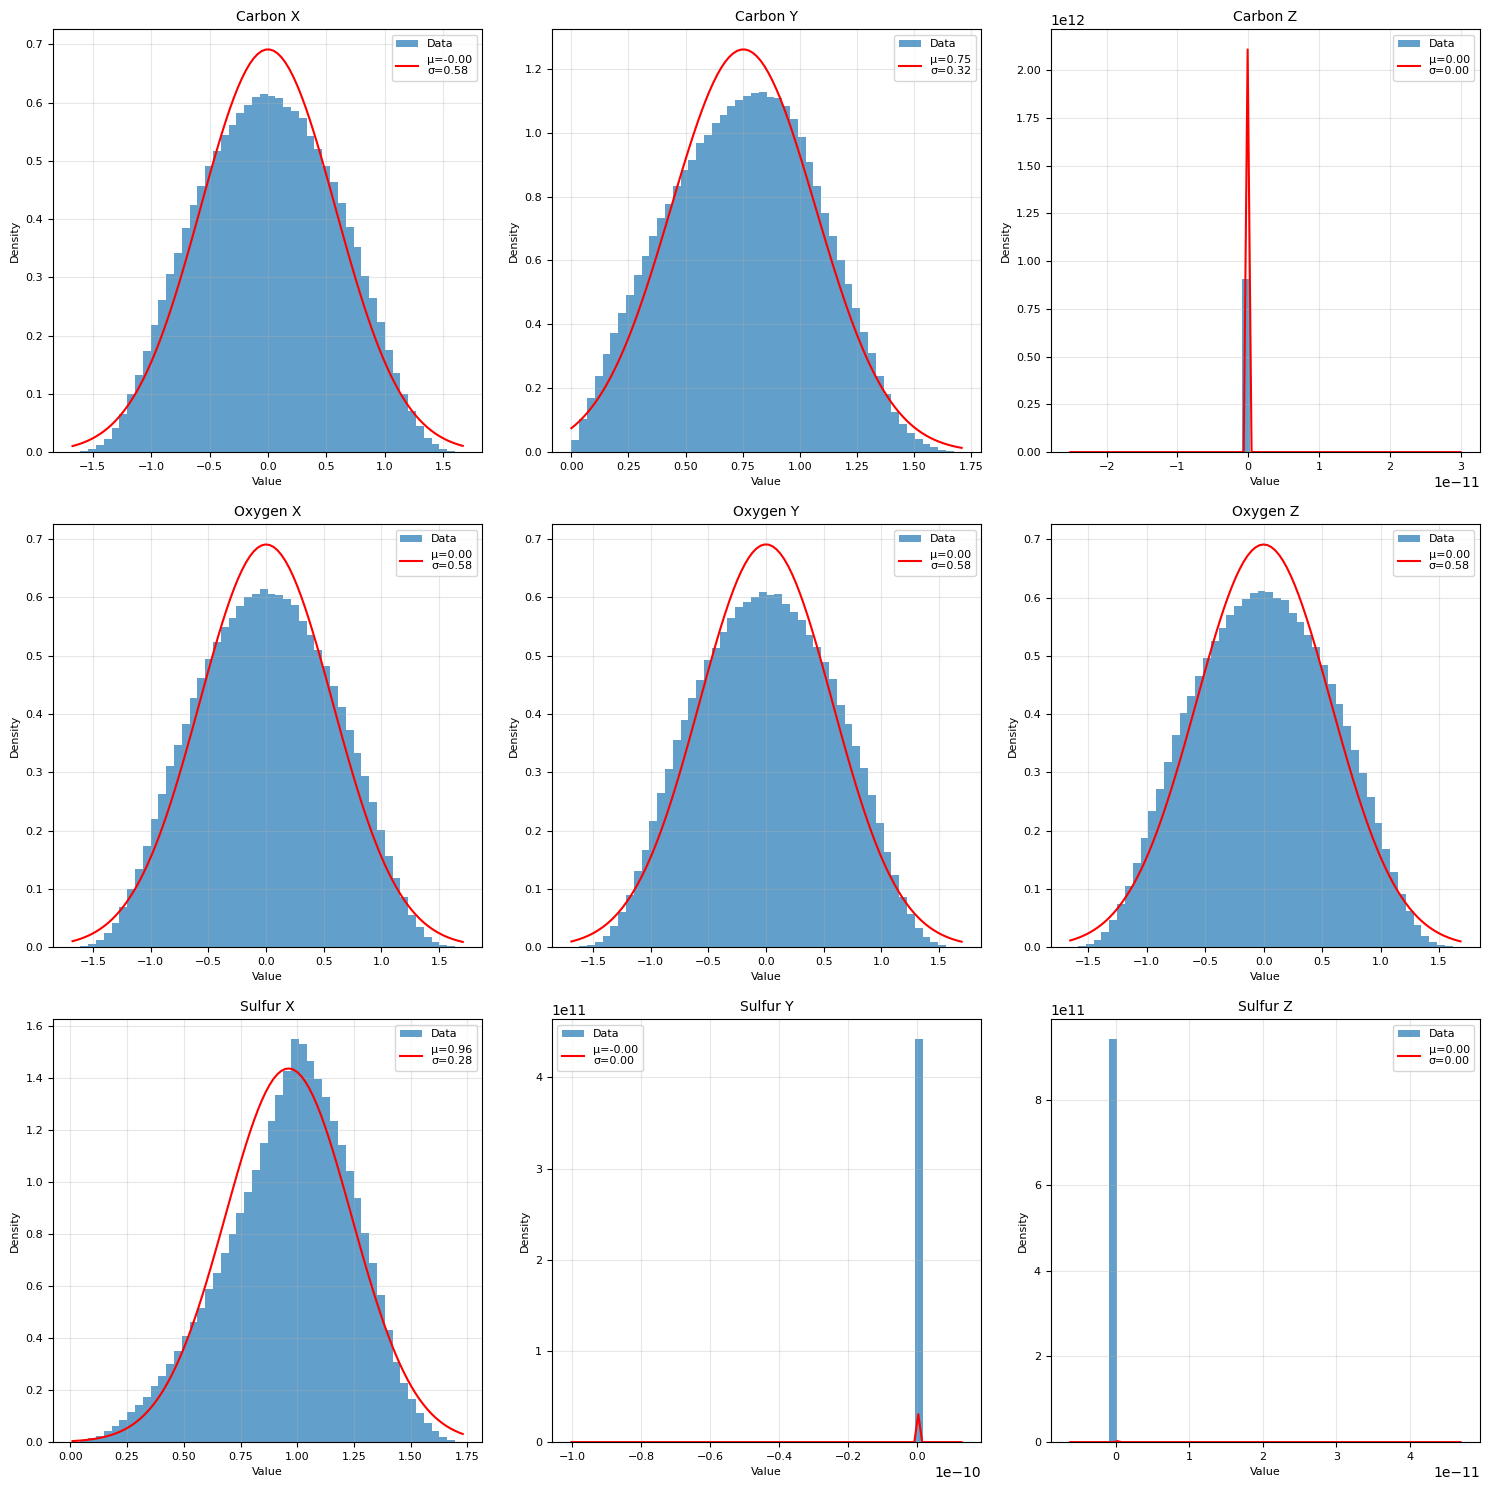
\includegraphics[width=1.2\textwidth]{random.png}
   \caption{Random 1M data}
\end{figure}

\begin{figure}[H]
   \centering
   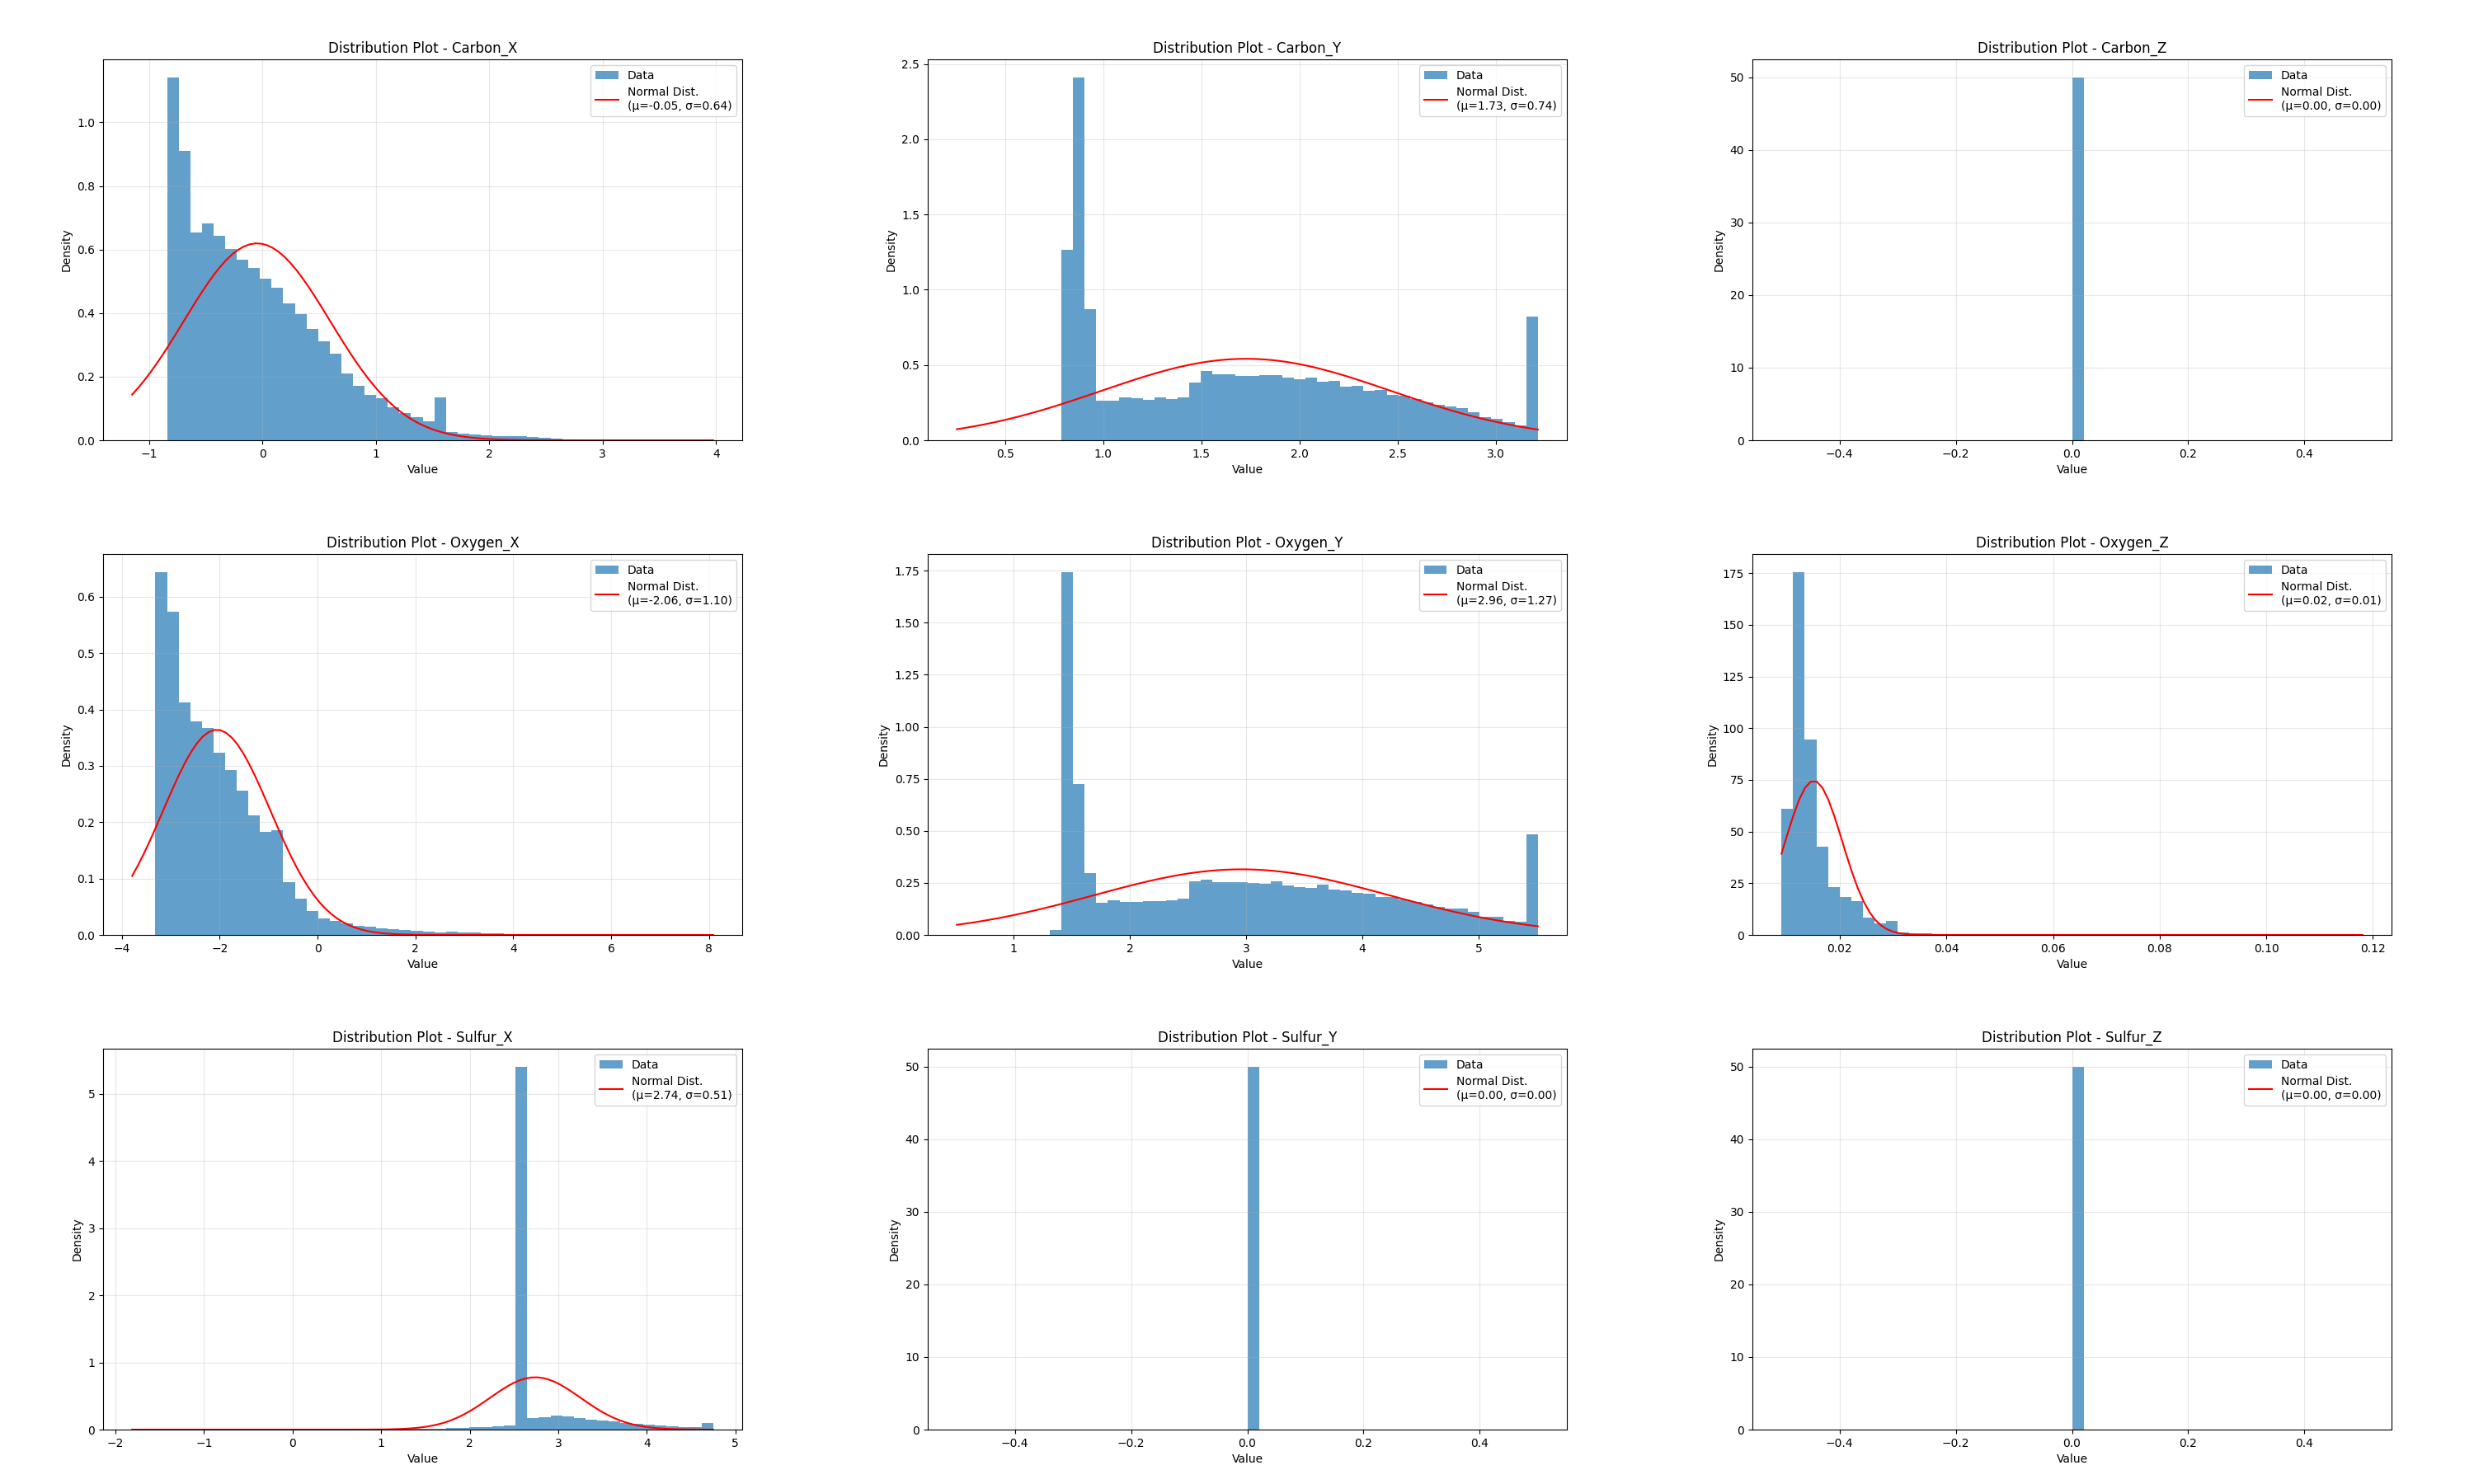
\includegraphics[width=1.2\textwidth]{EXP1.png}
   \caption{EXP1}
\end{figure}

\begin{figure}[H]
   \centering
   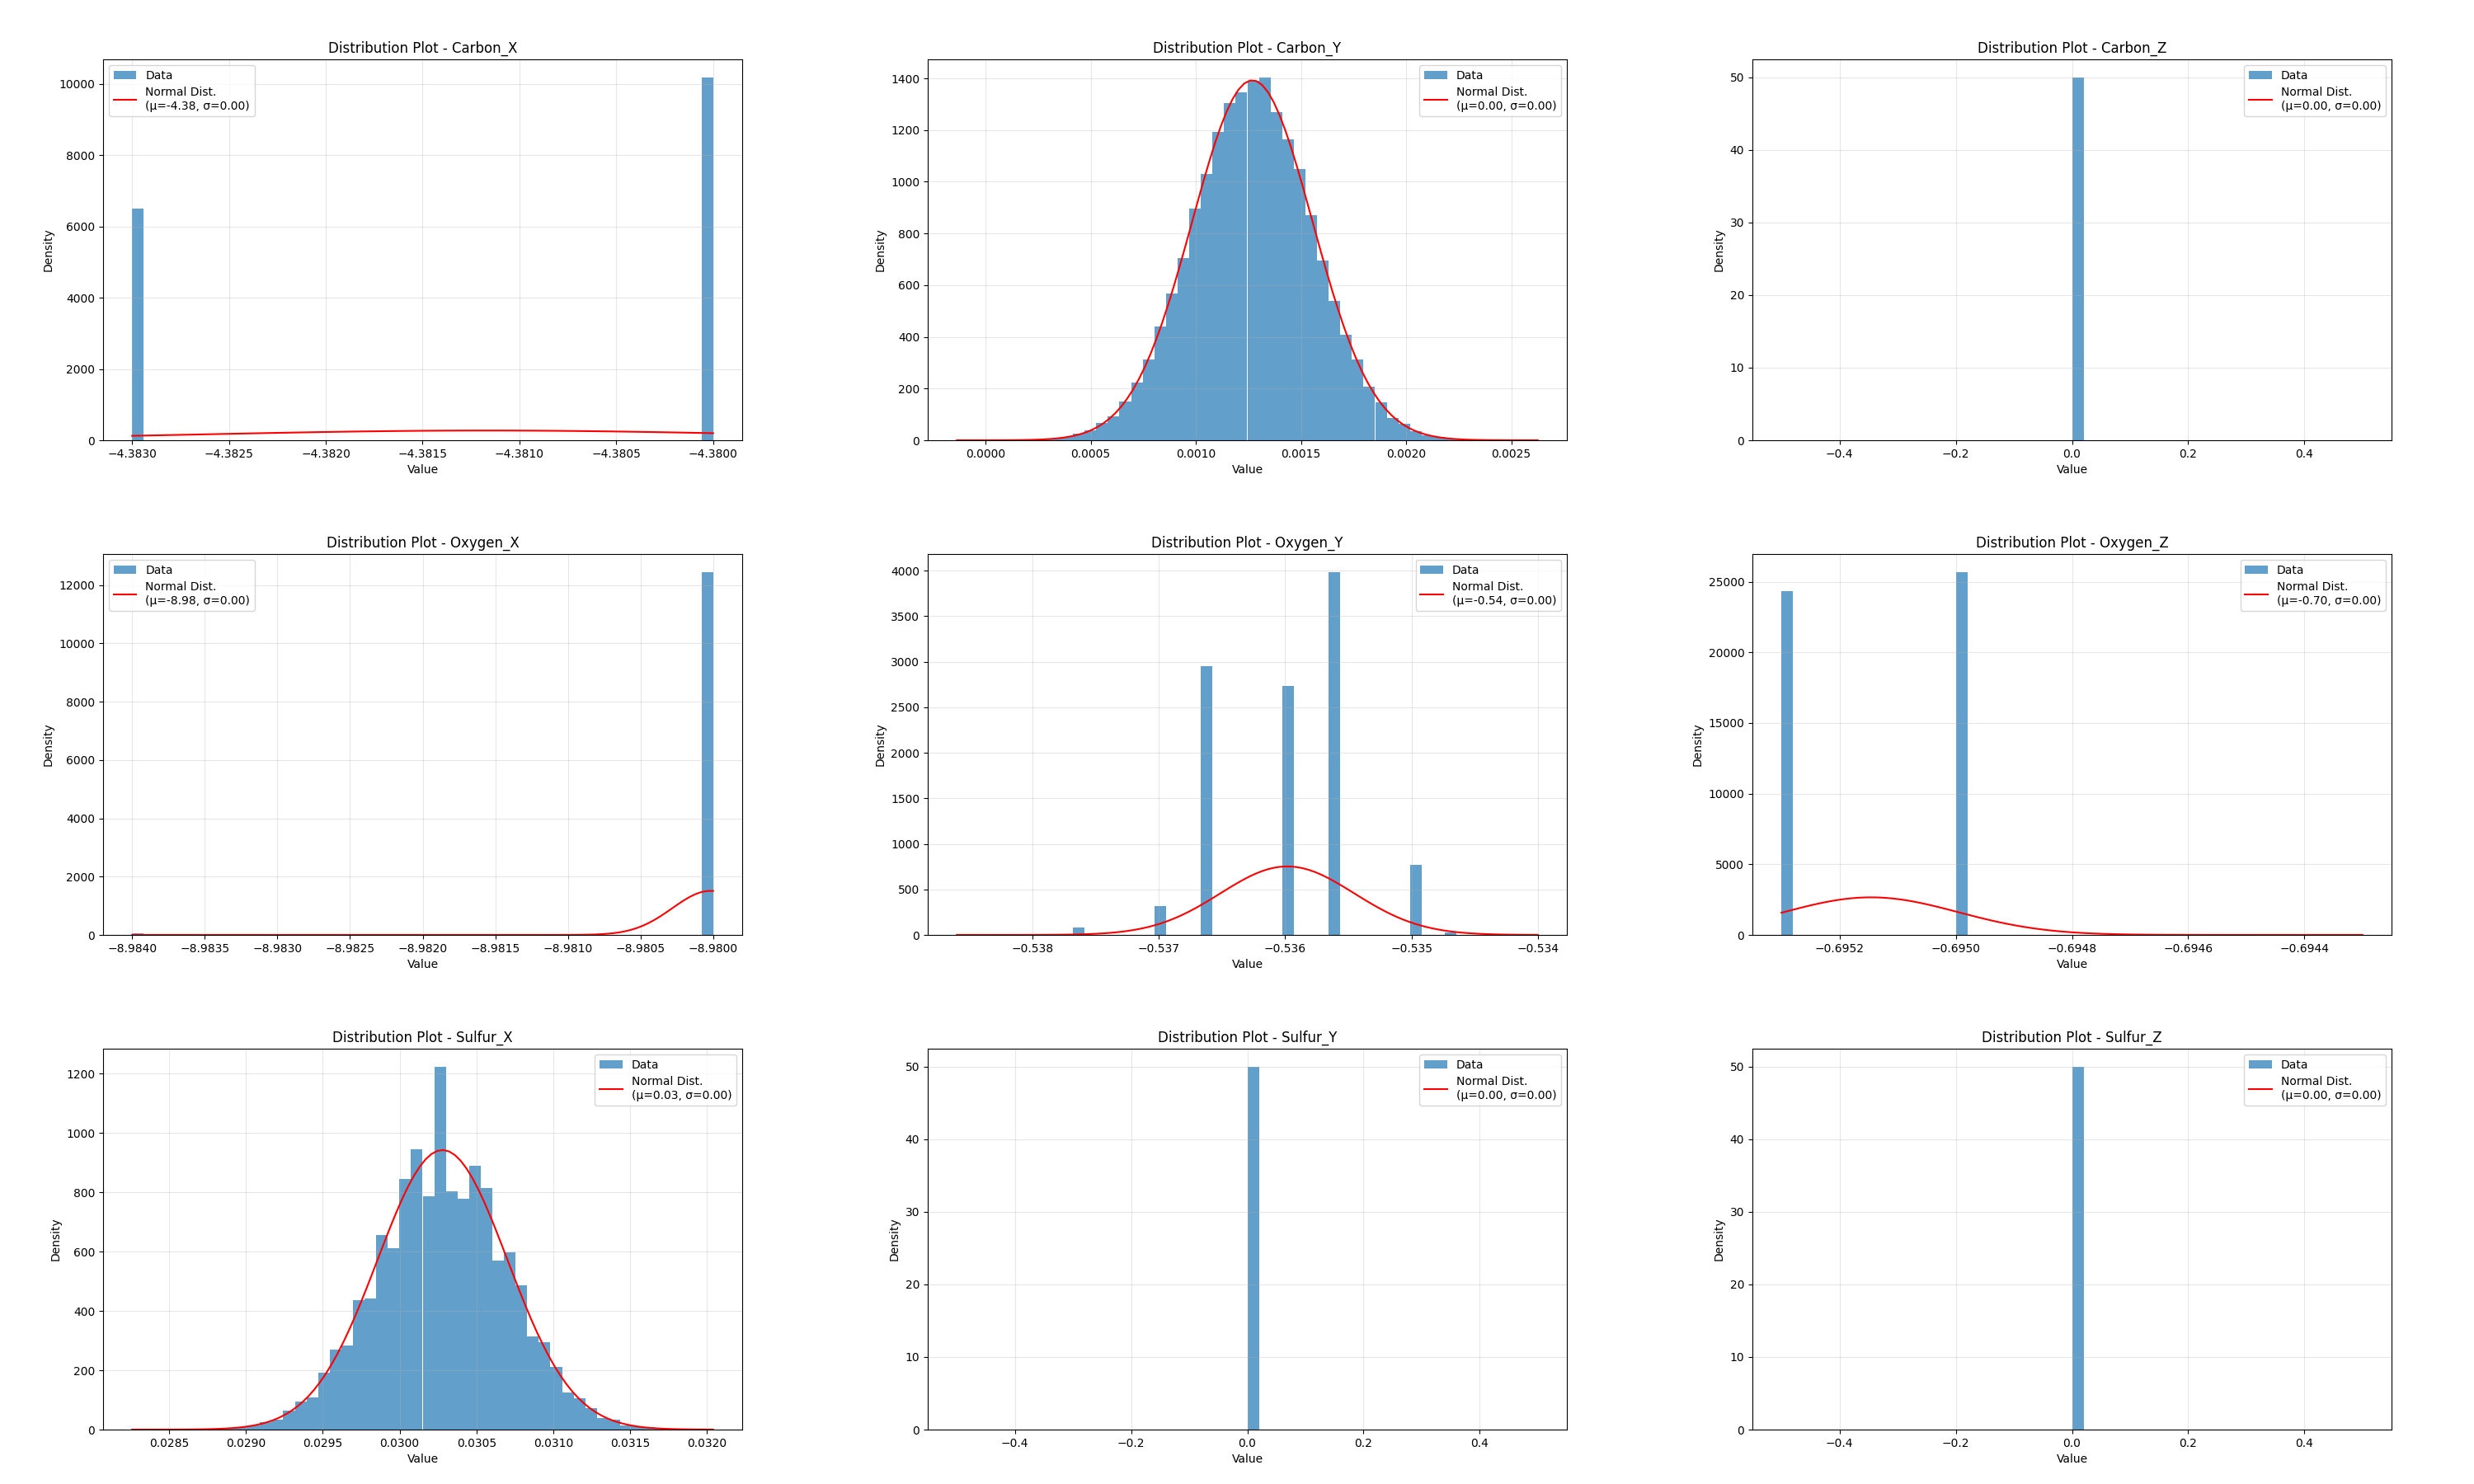
\includegraphics[width=1.2\textwidth]{EXP2.png}
   \caption{EXP2}
\end{figure}

\begin{figure}[H]
   \centering
   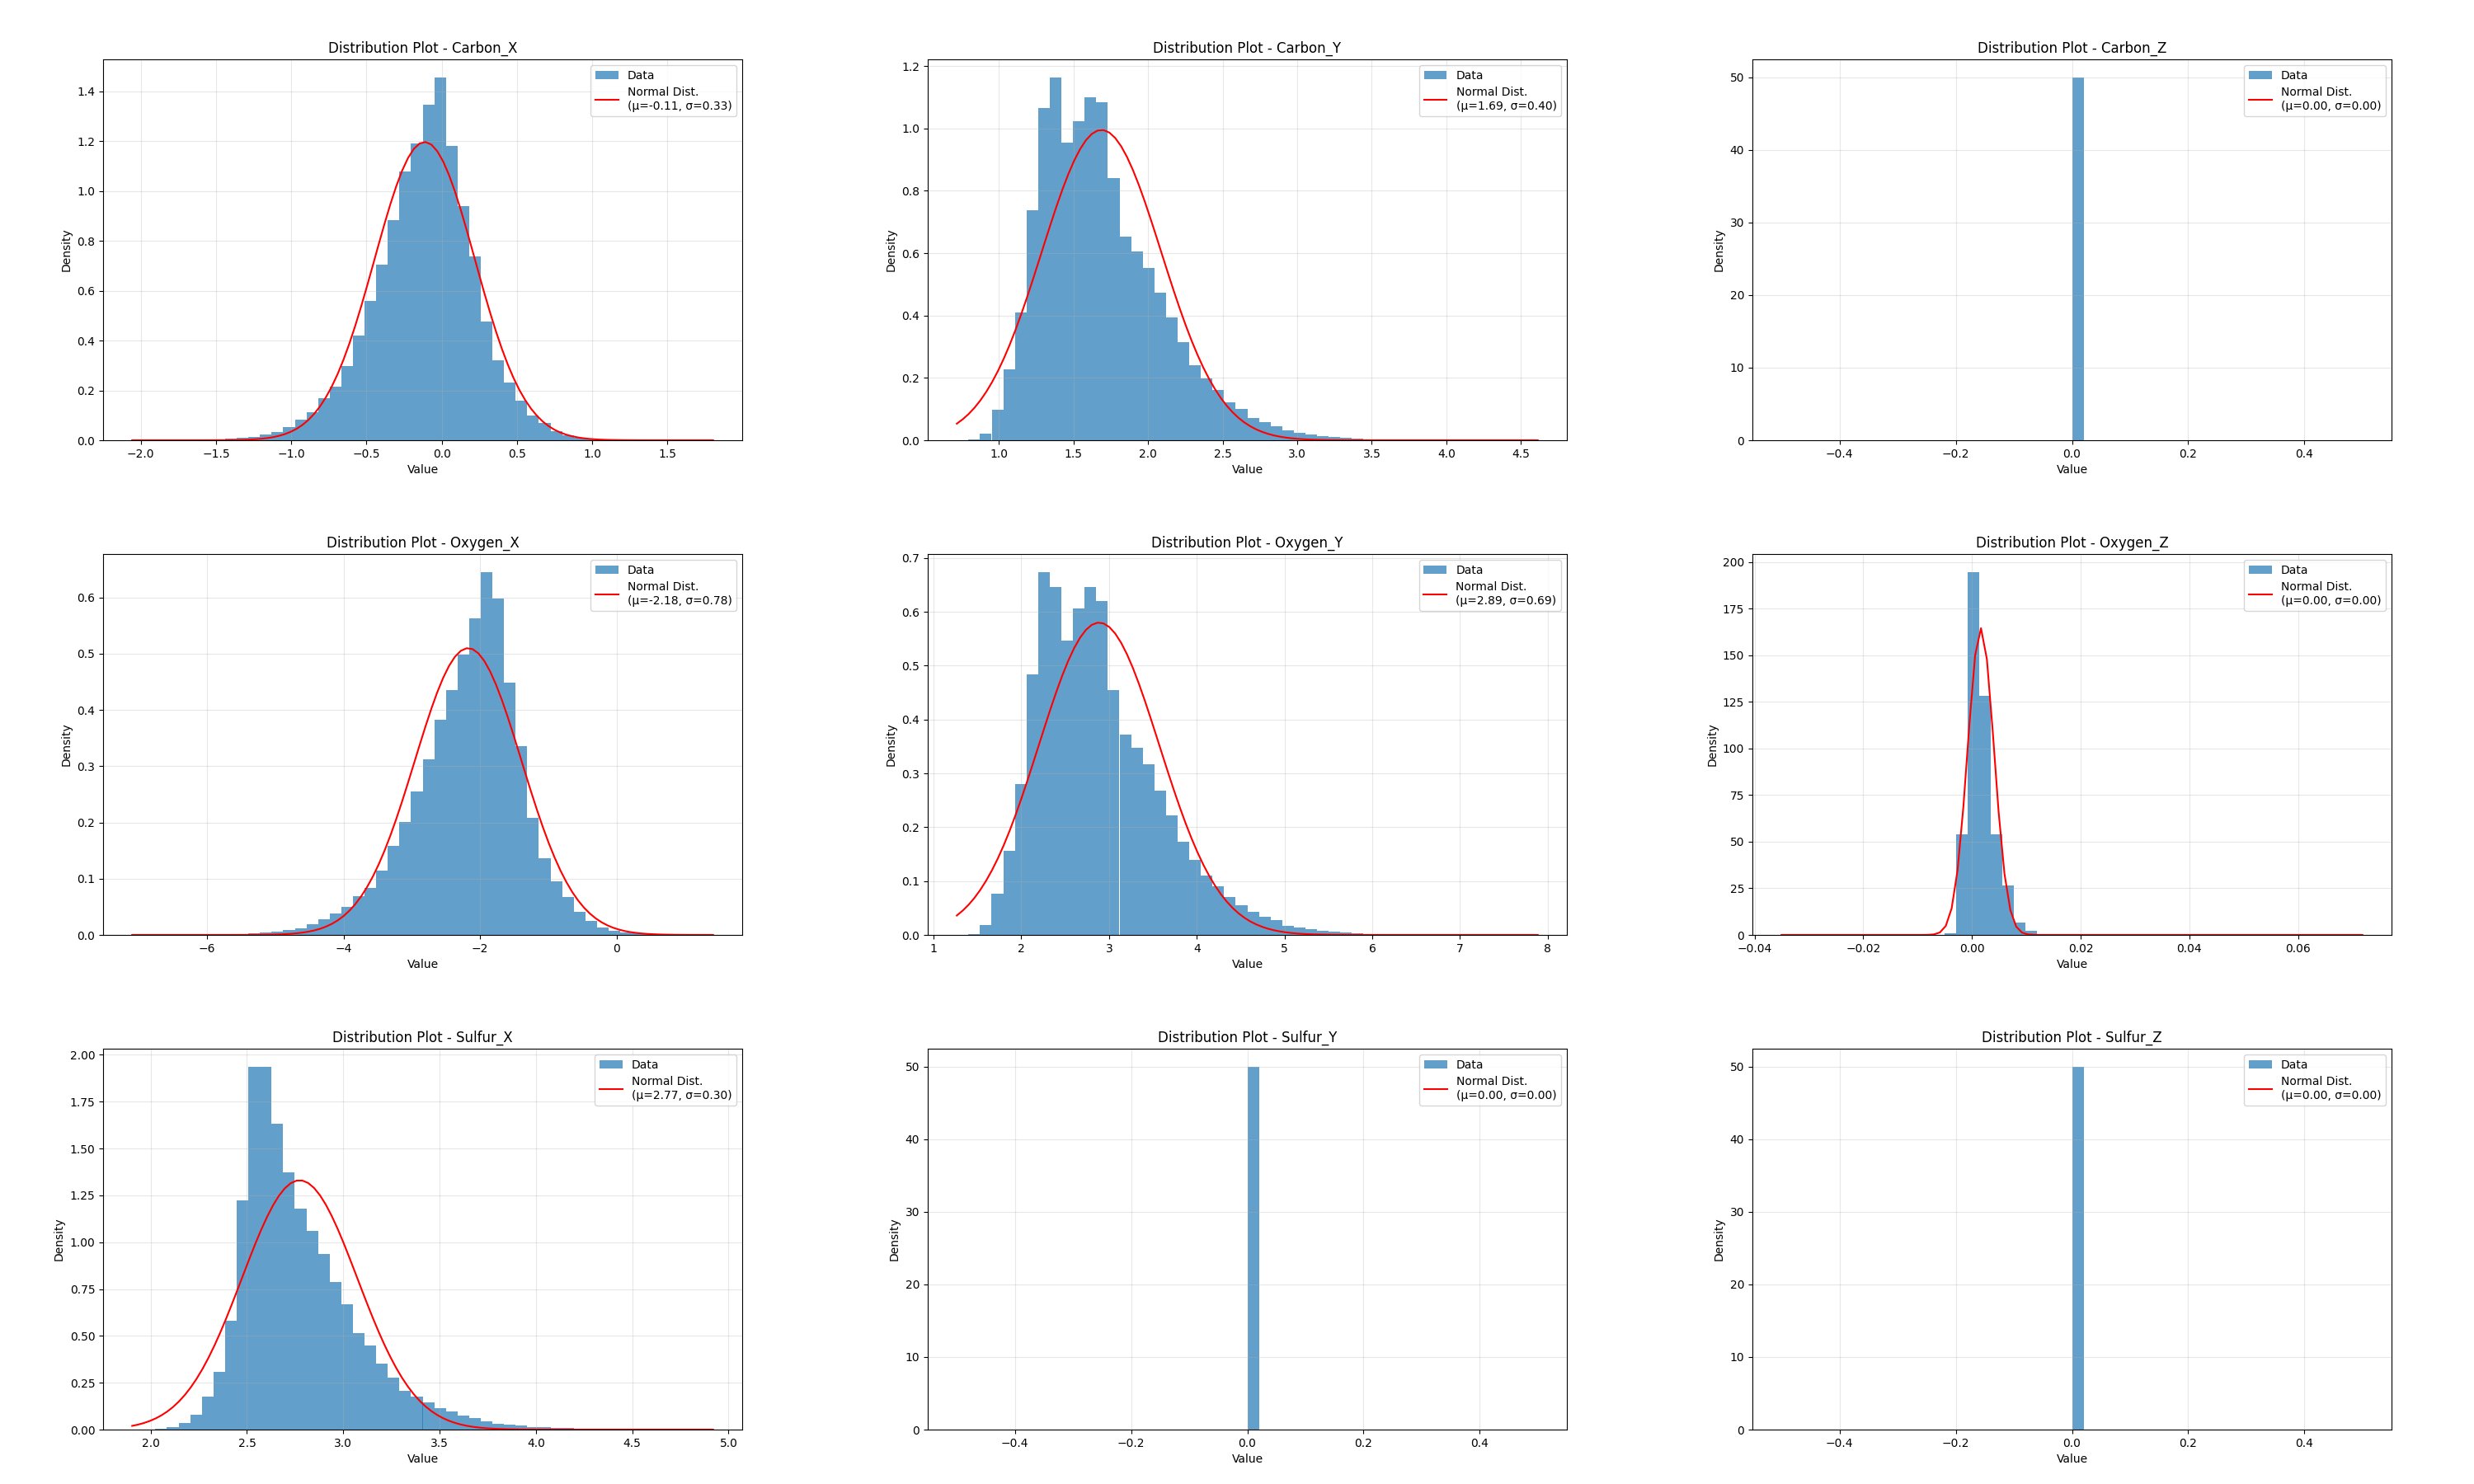
\includegraphics[width=1.2\textwidth]{EXP3.png}
   \caption{EXP3}
\end{figure}

\begin{figure}[H]
   \centering
   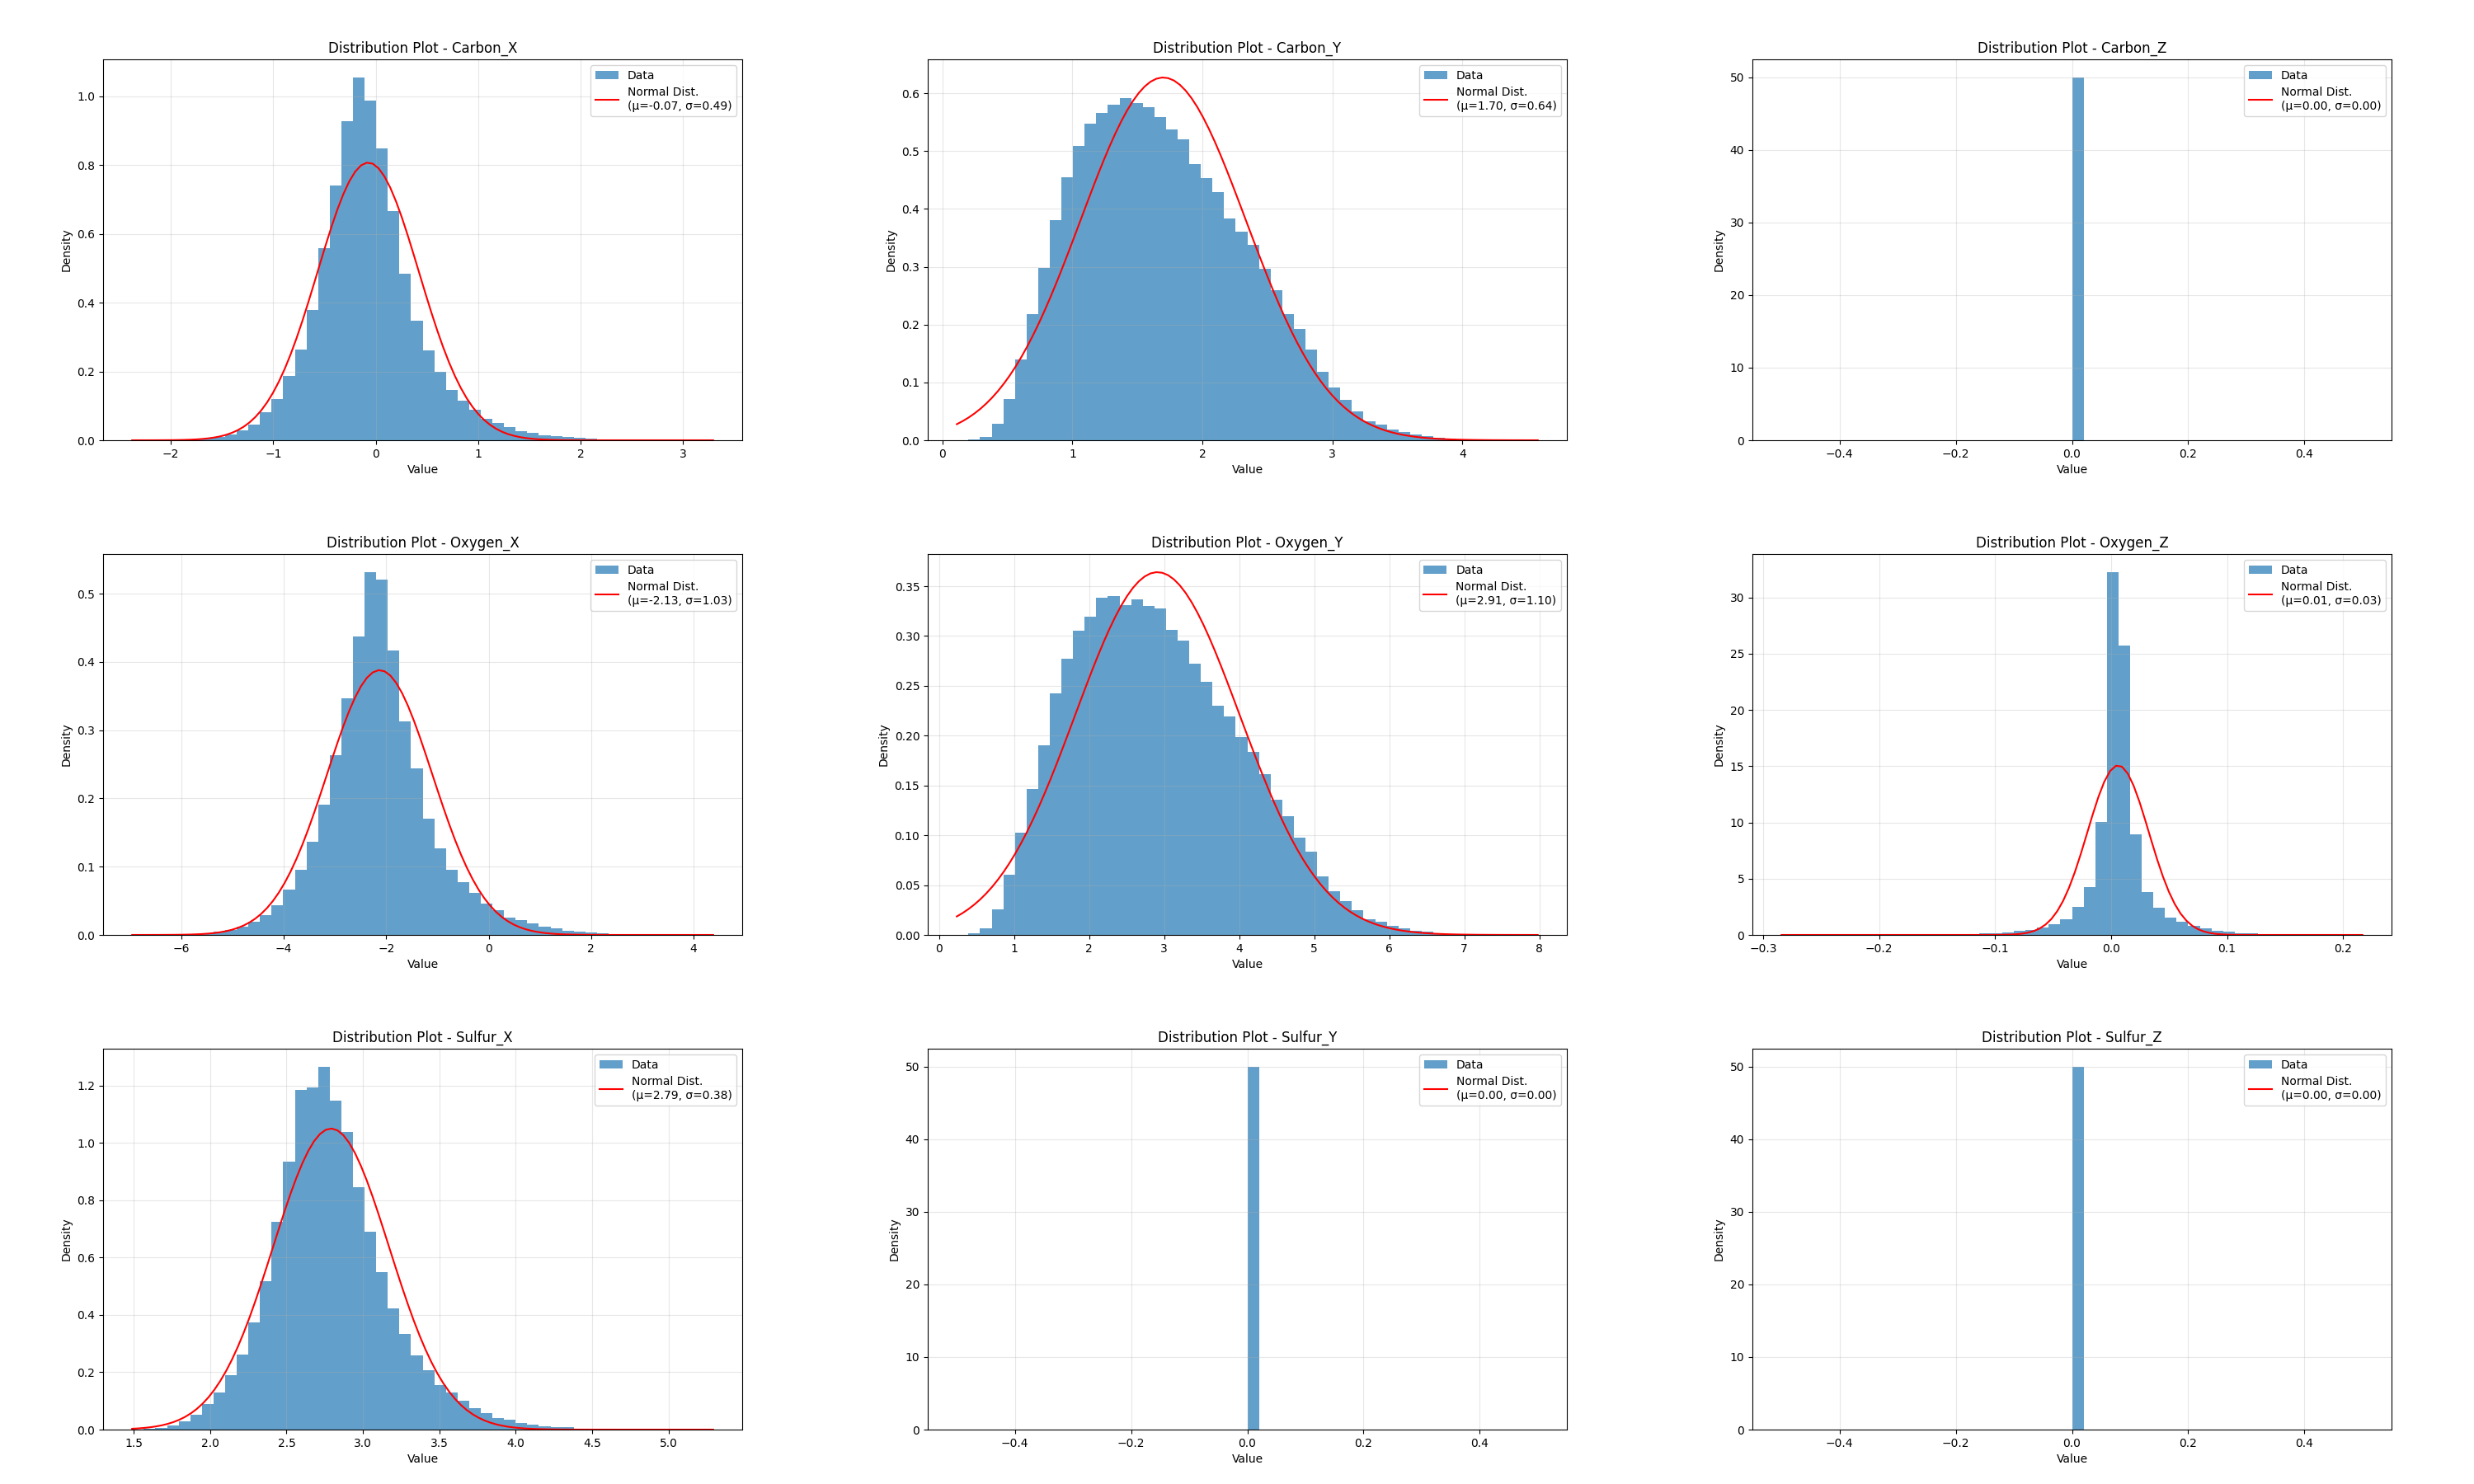
\includegraphics[width=1.2\textwidth]{EXP4.png}
   \caption{EXP4}
\end{figure}

\begin{figure}[H]
   \centering
   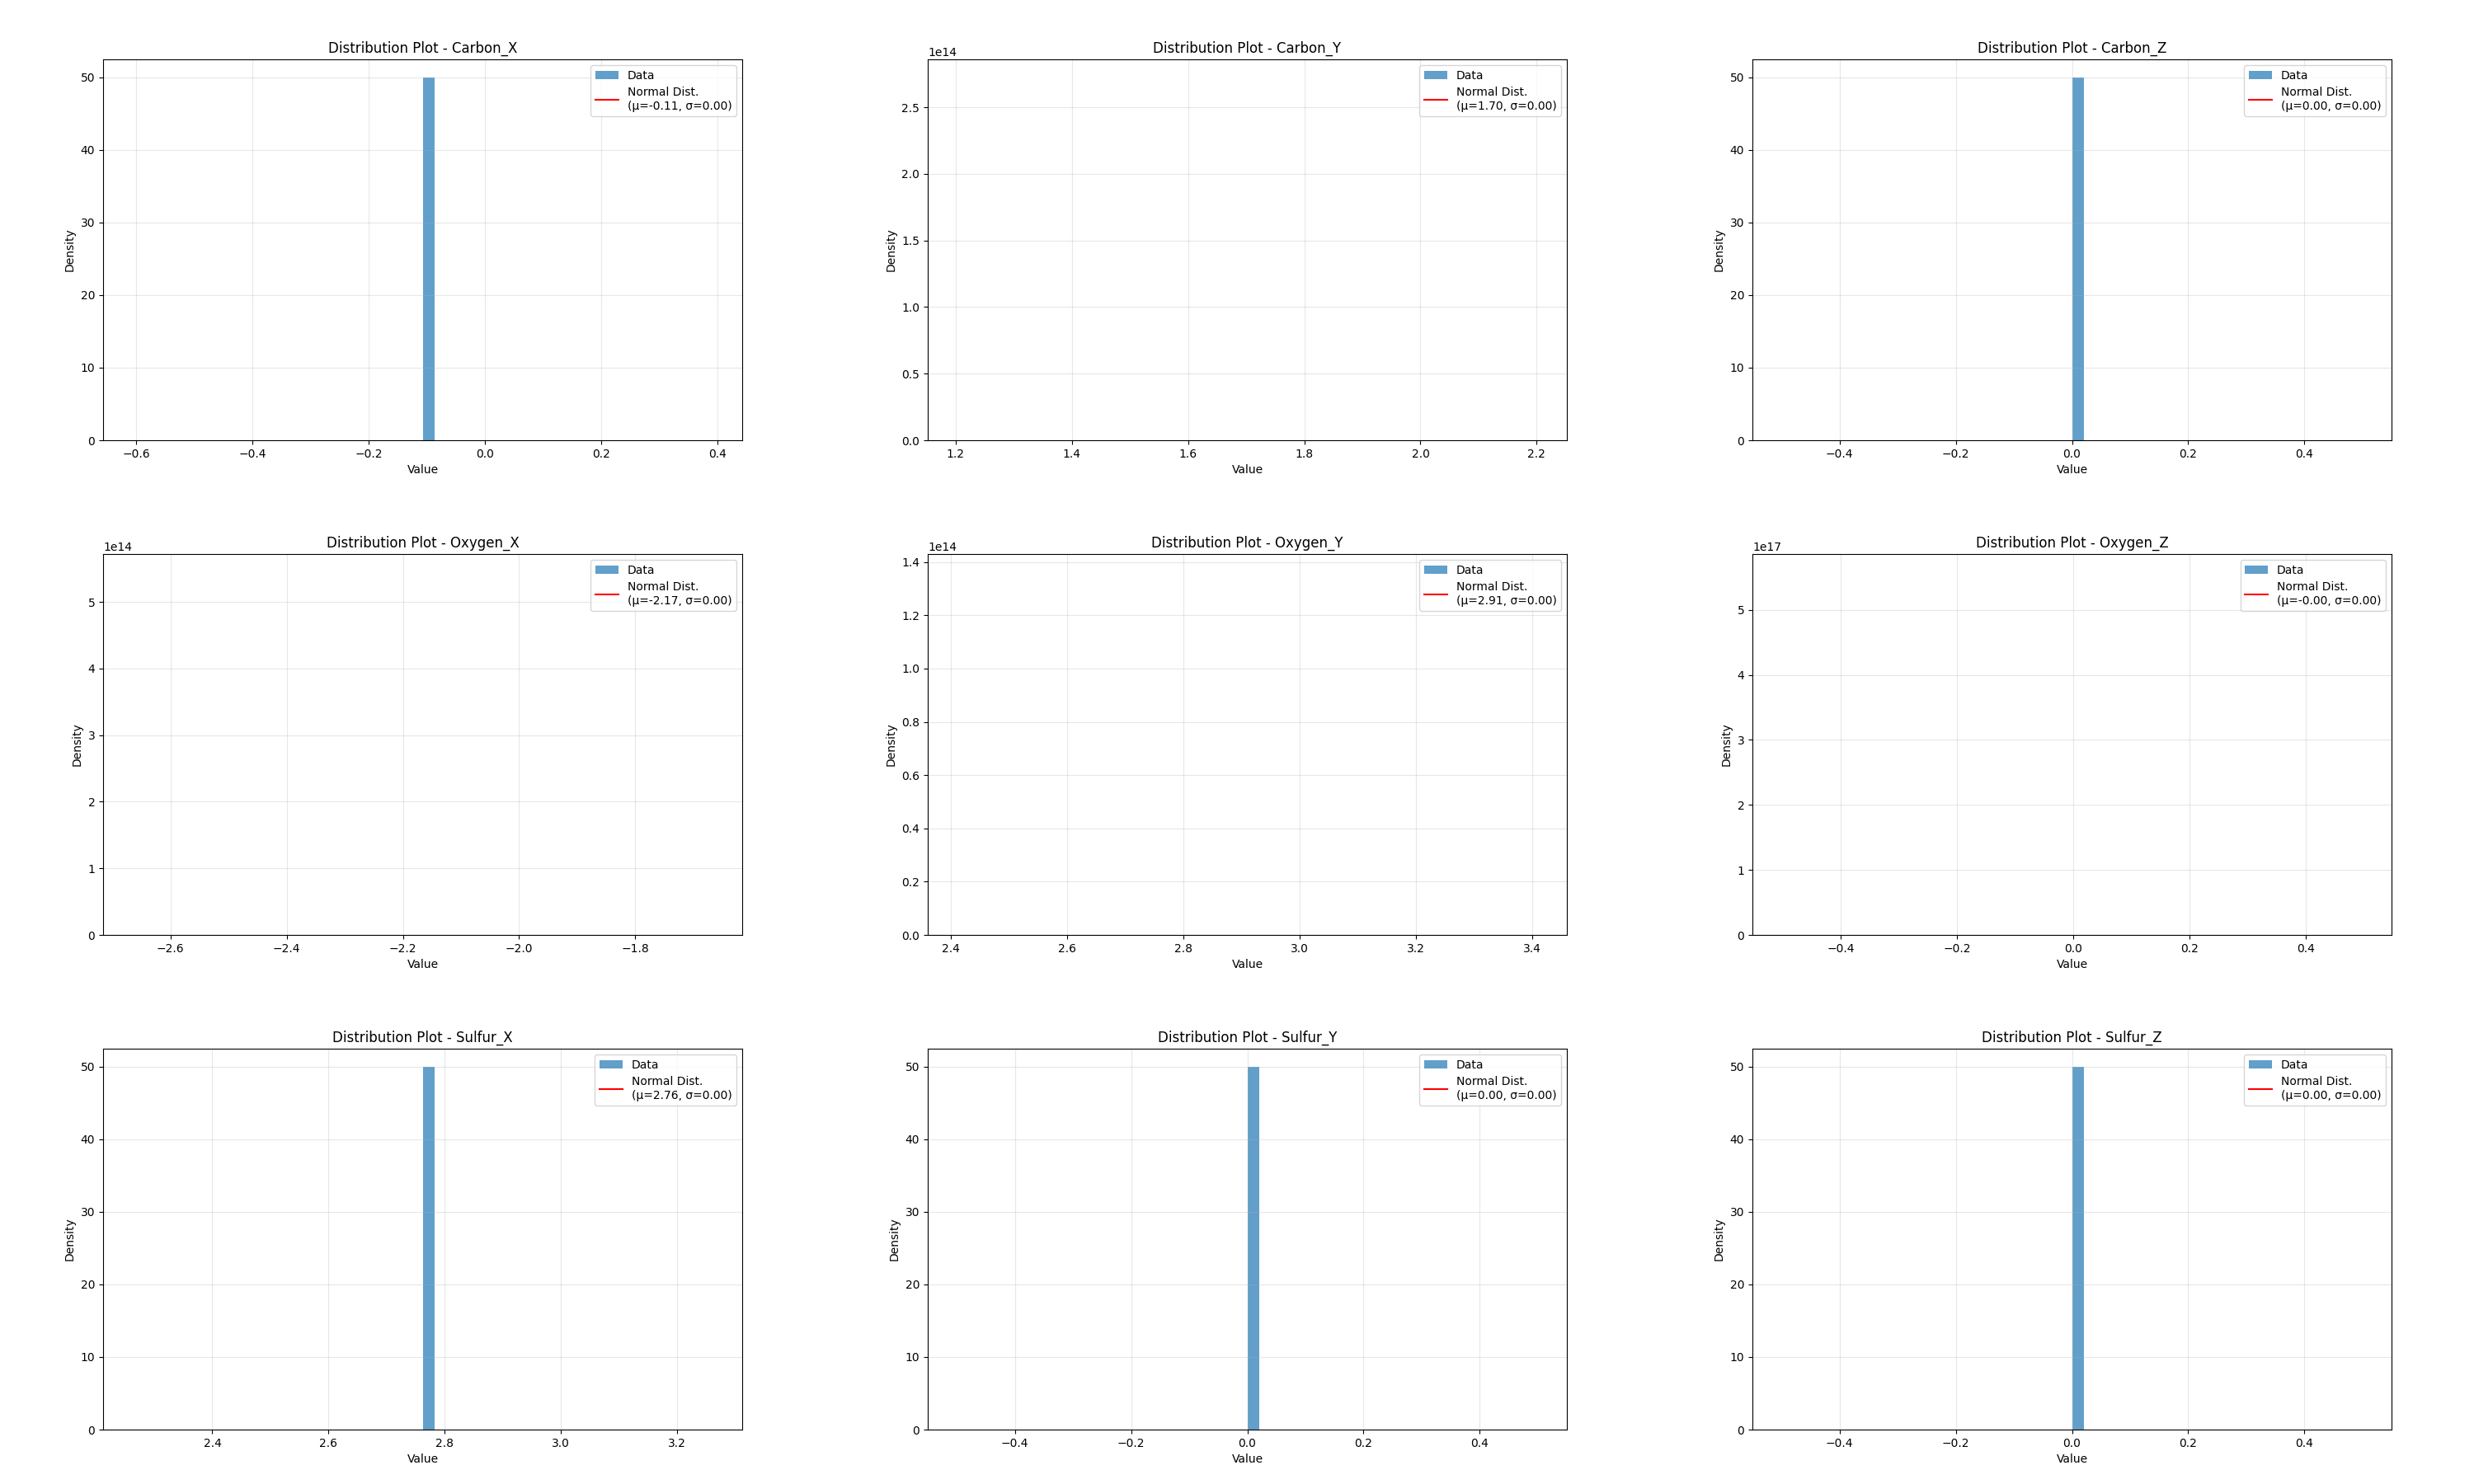
\includegraphics[width=1.2\textwidth]{EXP5.png}
   \caption{EXP5}
\end{figure}

\begin{figure}[H]
   \centering
   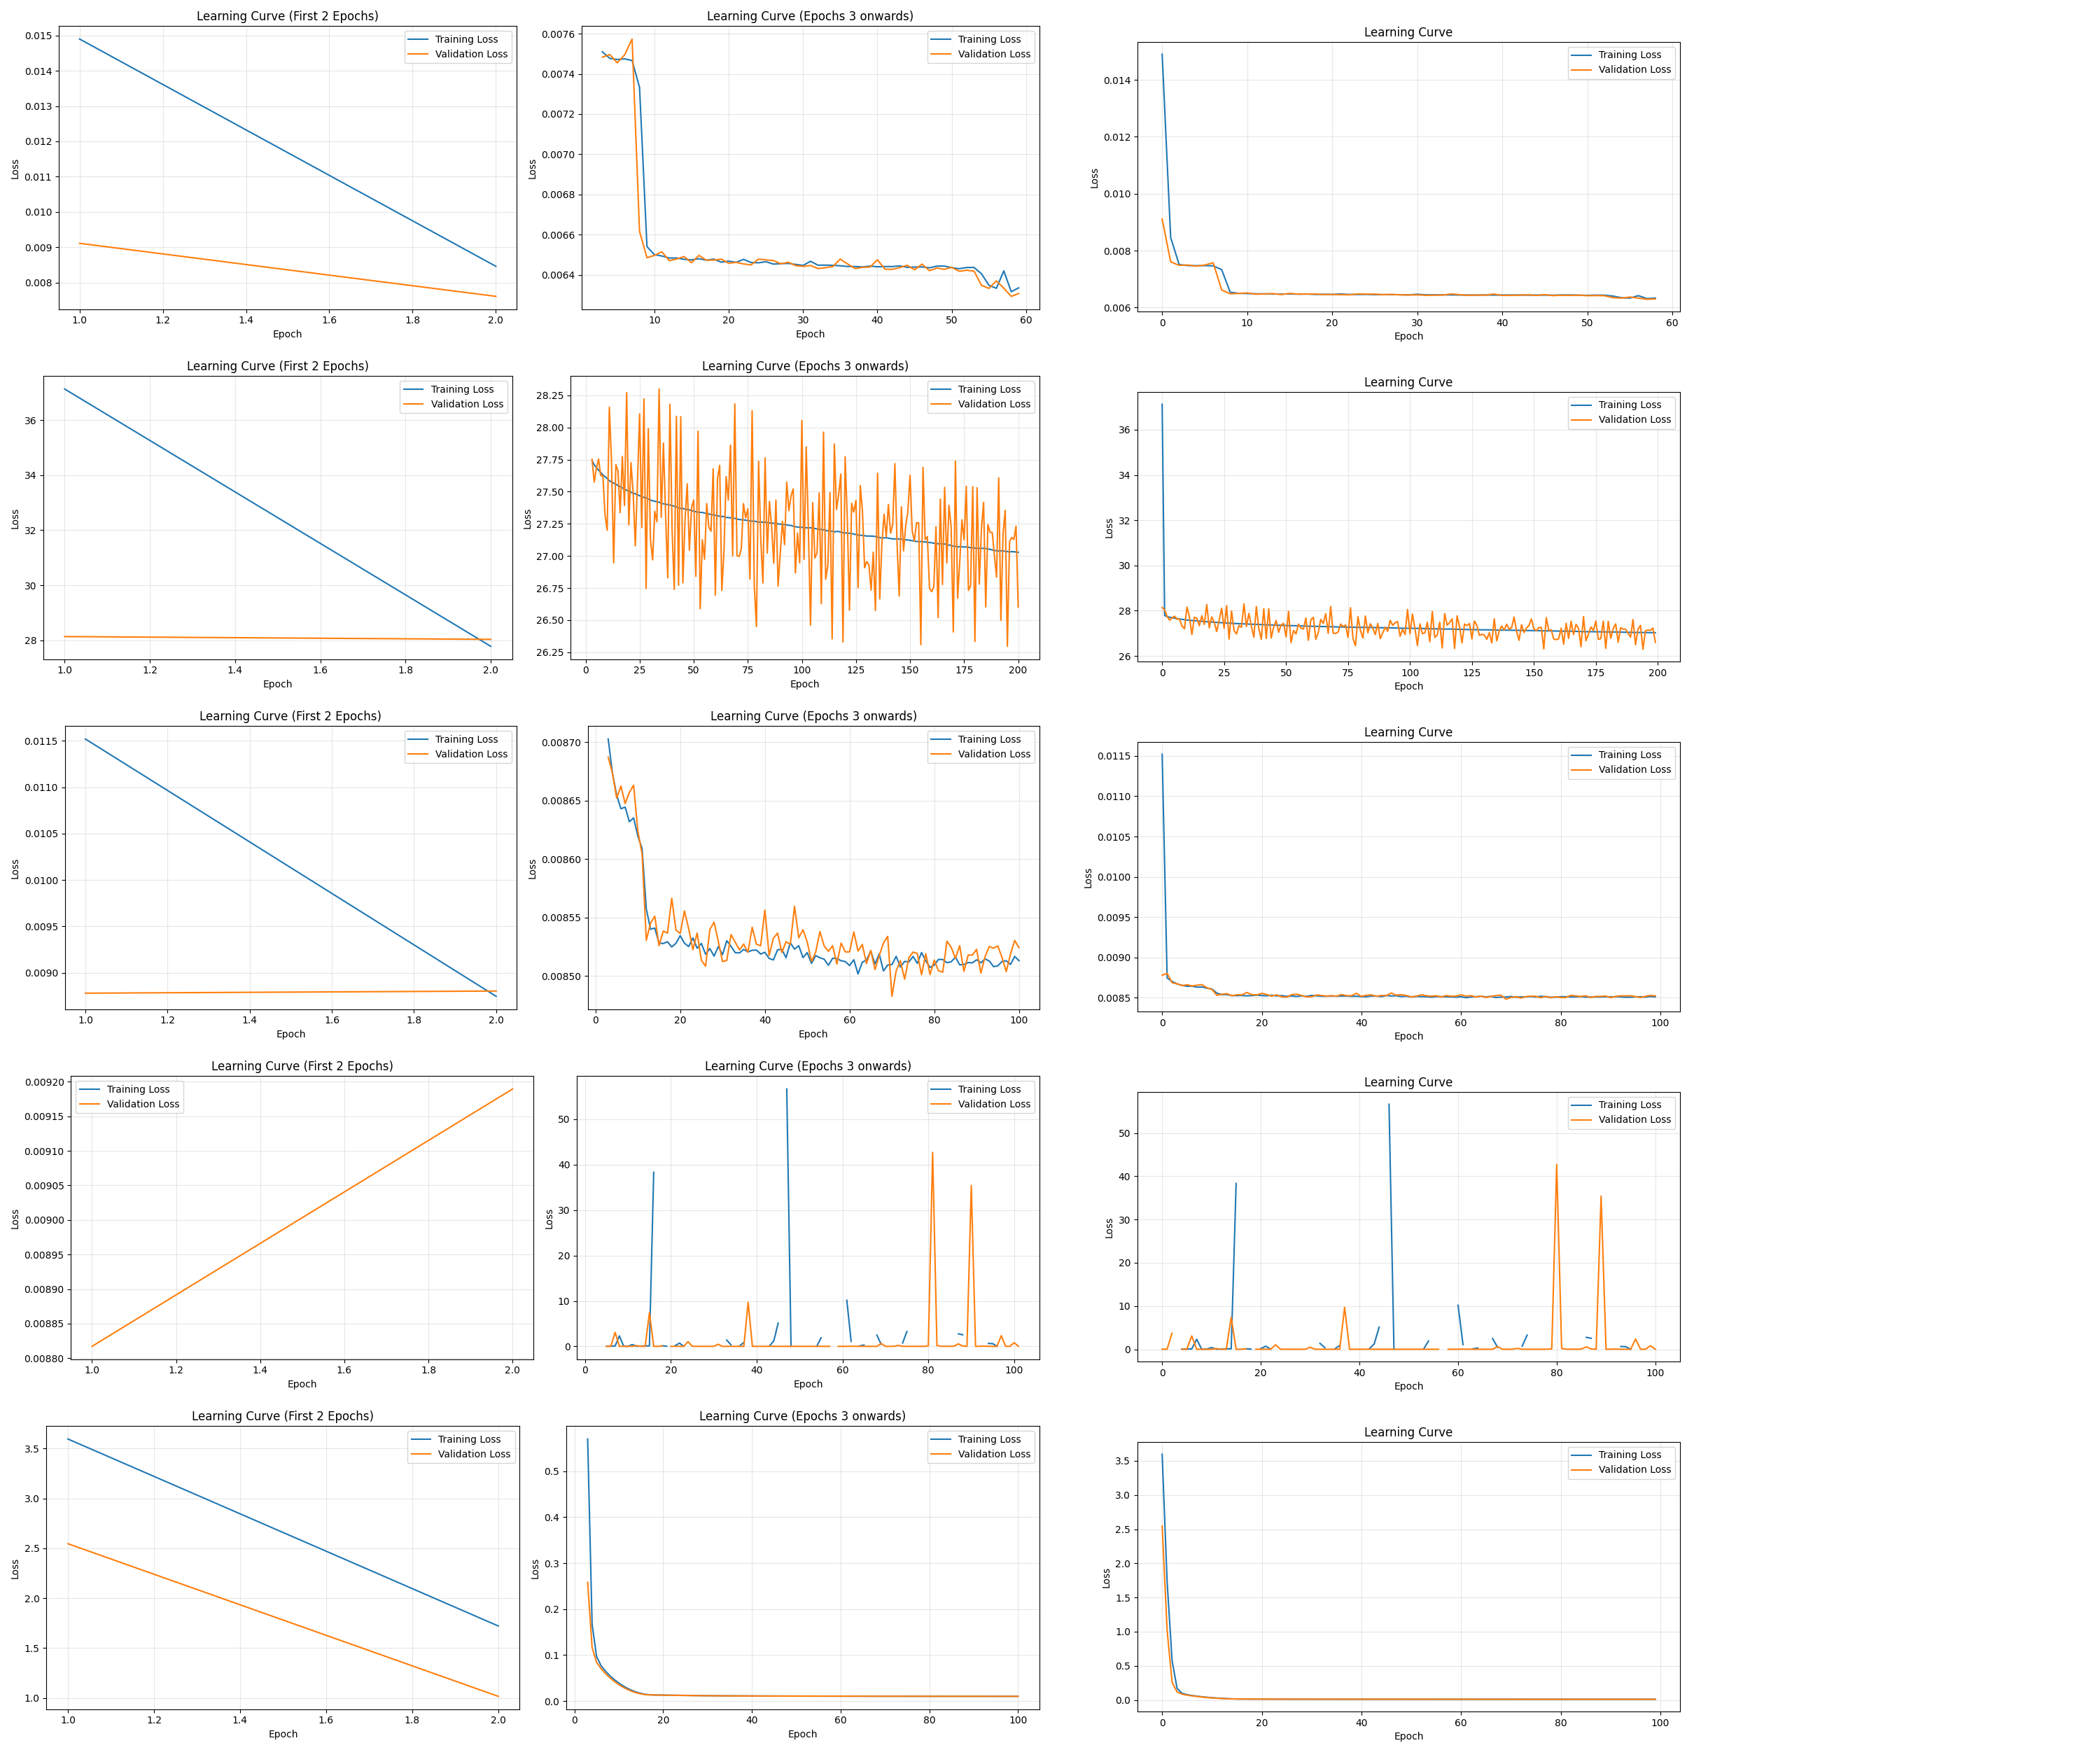
\includegraphics[width=1.4\textwidth]{LC.png}
   \caption{Learning curves, In order from EXP1 to EXP5}
\end{figure}




\begin{table}[ht]
\centering
\caption{Hyperparameter Configurations and Test MRE Results}
\begin{adjustbox}{max width=\textwidth}
\begin{tabular}{@{}lcccccccccccc@{}}
\toprule
\textbf{Test MRE} & \textbf{Latent Dim} & \textbf{Epochs} & \textbf{Batch Size} & \textbf{Learning Rate} & \textbf{Patience} & \textbf{Min Delta} & \textbf{Activation} & \textbf{Pos. Norm Method} & \textbf{Mom. Norm Method} & \textbf{L1} & \textbf{L2} & \textbf{Hidden Layers (Size)} \\ \midrule
0.2838           & 512                 & 200             & 1024                & 0.0098                 & 50                & 0.001              & ReLU               & MinMaxScaler             & MinMaxScaler            & No          & No          & 3 (256)                      \\
0.3379           & 256                 & 200             & 256                 & 0.0026                 & 100               & 0.01               & Tanh               & MinMaxScaler             & StandardScaler          & Yes         & No          & 1 (512)                      \\
0.3201           & 128                 & 100             & 128                 & 0.0002                 & 100               & 0.001              & ReLU               & MinMaxScaler             & MinMaxScaler            & No          & No          & 1 (512)                      \\
0.3157           & 256                 & 300             & 128                 & 0.00002                & 100               & 0.01               & ELU                & MinMaxScaler             & StandardScaler          & No          & No          & 2 (1024)                     \\
0.3109           & 256                 & 100             & 512                 & 0.00001                & 100               & 0.01               & ELU                & MinMaxScaler             & MinMaxScaler            & Yes         & Yes         & 4 (512)                      \\ \bottomrule
\end{tabular}
\end{adjustbox}
\label{tab:hyperparameters}
\end{table}

\end{document}

